\documentclass{beamer}
\usetheme{metropolis}           % Use metropolis theme
\usepackage{graphicx} % For including images
\usepackage{url} % For handling URLs
\usepackage{tcolorbox} % For creating pretty boxes

% Define a custom tcolorbox style for definitions
\tcbset{
    definitionstyle/.style={
        colback=blue!5!white, % Background color
        colframe=blue!75!black, % Border color
        fonttitle=\bfseries, % Bold title
        coltitle=white, % Title color
        boxrule=0.75mm, % Border thickness
        arc=2.5mm, % Rounded corners
        left=2mm, % Left padding
        right=2mm, % Right padding
        top=1mm, % Top padding
        bottom=1mm % Bottom padding
    }
}

% for the sources of images: very small footnotes
\newcommand{\sourcefootnote}[1]{\let\thefootnote\relax\footnote{{\tiny Source: \url{#1}}}}

\title{Temporal Graphs}

\date{\today}

\author{Daniel Cermann}

\institute{
  \hfill \begin{minipage}{0.3\textwidth}
    \begin{center}
      
\includegraphics[width=60px]{media/hpi_logo.png} \newline
      Hasso Plattner Institute 
    \end{center}
  \end{minipage}
}


\begin{document}

\begin{frame}
  \begin{center}
    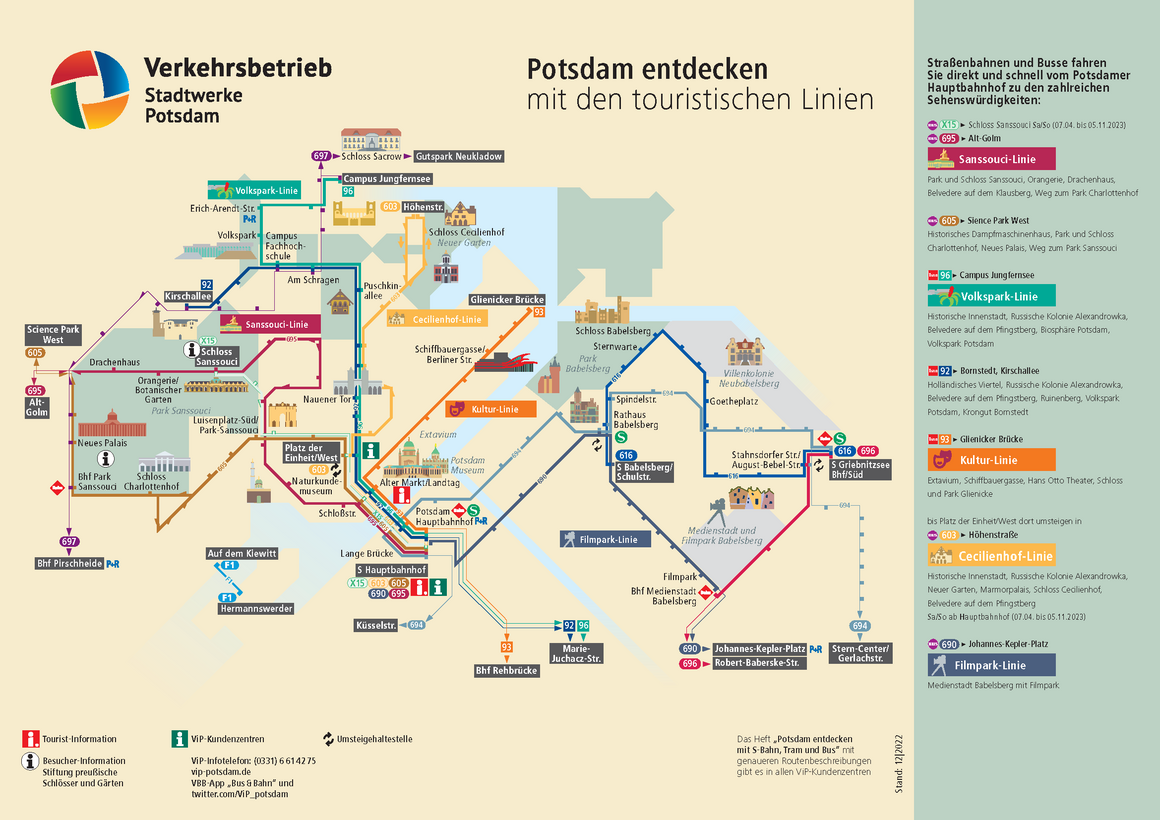
\includegraphics[width=0.95\textwidth]{media/potsdam_citynet.png}
  \end{center}
  \sourcefootnote{https://www.swp-potsdam.de/content/verkehr/bilder_6/liniennetz/touristischer_liniennetzplan_screenshot_1280_960.jpg}
\end{frame}

\maketitle

\section{Motivation}


% insert some real-live applications here


\begin{frame}{Definition}
    \begin{tcolorbox}[definitionstyle, title=Definition]
        A \textbf{labeled graph} \cite{GHOSH201888} is a graph \( G = (V, E) \) where:
        \begin{itemize}
            \item \( V \) is the set of vertices, each assigned a unique label.
            \item \( E \subseteq \{(u, v) \mid u, v \in V\} \) is the set of edges, where edges may also have labels.
          \end{itemize}
    \end{tcolorbox}
\end{frame}


\begin{frame}{Sources}
  \bibliographystyle{plain}
  \bibliography{references}
\end{frame}

\end{document}
